\documentclass[12pt]{article}

\usepackage[margin=1in]{geometry}
\usepackage{amsmath,amsthm,amssymb}
\usepackage{nccmath}
\usepackage{mathtools}
\usepackage{mathrsfs}
\usepackage{enumitem}
\usepackage{physics}
\usepackage{tensor}
\usepackage{subcaption}
\usepackage{pdfpages}
\usepackage{graphicx}
\graphicspath{ {./images/} }

\usepackage{tikz}
\usetikzlibrary{calc,decorations.markings,patterns}

\newcommand{\chrissym}[3]{\Gamma_{#2#3}^#1}

\begin{document}

\title{Midterm}
\author{Sean Ericson \\ Phys 610}
\maketitle

\section*{Problem 1}
The metric and its inverse are given by:
\begin{align*}
    g_{\mu\nu} &= \mqty(-\left(1 - \frac{2M}{\sqrt{r^2 + b^2}}\right) & 0 & 0 & 0 \\ 0 & \left(1 - \frac{2M}{\sqrt{r^2 + b^2}}\right)^{-1} & 0 & 0 \\ 0 & 0 & r^2 + b^2 & 0 \\ 0 & 0 & 0 & (r^2 + b^2)\sin^2\theta) \\
    g^{\mu\nu} &= \mqty(-\left(1 - \frac{2M}{\sqrt{r^2 + b^2}}\right)^{-1} & 0 & 0 & 0 \\ 0 & \left(1 - \frac{2M}{\sqrt{r^2 + b^2}}\right) & 0 & 0 \\ 0 & 0 & \frac{1}{r^2 + b^2} & 0 \\ 0 & 0 & 0 & \frac{1}{(r^2 + b^2)\sin^2\theta}) \\
\end{align*}


\section*{Problem 2}
The Christoffel symbols were calculated using the attached Mathematica code. Their reduction to those of the Schwarzschild metric when $b \to 0$ is clear.
\begin{align*}
    \chrissym{t}{t}{r} &= \frac{M}{r^2 + b^2}\left(1 - \frac{2M}{\sqrt{r^2 + b^2}}\right)^{-1} \\
    \chrissym{r}{t}{t} &= \frac{Mr}{(r^2 + b^2)^\frac{3}{2}}\left(1 - \frac{2M}{\sqrt{r^2 + b^2}}\right) \\
    \chrissym{r}{r}{r} &= -\frac{M}{r^2 + b^2}\left(1 - \frac{2M}{\sqrt{r^2 + b^2}}\right)^{-1} \\
    \chrissym{r}{\theta}{\theta} &= -r\left(1 - \frac{2M}{\sqrt{r^2 + b^2}}\right) \\
    \chrissym{r}{\phi}{\phi} &= -r\left(1 - \frac{2M}{\sqrt{r^2 + b^2}}\right) \sin^2\theta \\
    \chrissym{\theta}{\theta}{r} &= \frac{r}{r^2 + b^2}  \\
    \chrissym{\theta}{\phi}{\phi} &= -\sin\theta\cos\theta \\
    \chrissym{\phi}{\phi}{r} &= \frac{r}{r^2 + b^2} \\
    \chrissym{\phi}{\phi}{\theta} &= \cot\theta
\end{align*}

\section*{Problem 3}
The geodesic equations were calculated with the attached Mathematica code.
\begin{align*}
    \ddot{t} &= -\frac{2Mr}{(r^2 + b^2)^\frac{3}{2}}\left(1 - \frac{2M}{\sqrt{r^2 + b^2}}\right)\dot{t}\dot{r} \\
    \ddot{r} &= r\left(1 - \frac{2M}{\sqrt{r^2 + b^2}}\right)\left(\sin^2\theta\dot{\phi}^2 + \dot{\theta}^2\right) - \left(1 - \frac{2M}{\sqrt{r^2 + b^2}}\right)\frac{Mr\dot{t}^2}{(r^2 + b^2)^\frac{3}{2}} + \left(1 - \frac{2M}{\sqrt{r^2 + b^2}}\right)^{-1}\frac{Mr\dot{r}^2}{(r^2 + b^2)^\frac{3}{2}}\\
    \ddot{\theta} &= \sin\theta\cos\theta\dot{\phi}^2 - \frac{2r\dot{\theta}\dot{r}}{r^2 + b^2} \\
    \ddot{\phi} &= -2\dot{\phi}\left(\cot\theta\dot{\theta} + \frac{r\dot{r}}{r^2 + b^2}\right)
\end{align*}


\section*{Problem 4}
The metric is independent of $t$ and $\phi$, so we have two conserved quantities:
\begin{align*}
    e &\coloneqq -\xi_t^{\;\mu}u_\mu = \left(1 - \frac{2M}{\sqrt{r^2 + b^2}}\right)\dot{t} \\
    l &\coloneqq -\xi_\phi^{\;\mu}u_\mu = -(r^2 + b^2)\sin^2\theta\dot{\phi}
\end{align*}
The $\phi$ independence also implies that orbits lie in a plane, so we can consider an orbit in the $\theta = \pi/2$ plane, with $\dd\theta = 0$.
\begin{alignat}{3}
    & & u^2 = -1 &= -\left(1 - \frac{2M}{\sqrt{r^2 + b^2}}\right)\dot{t}^2 + \left(1 - \frac{2M}{\sqrt{r^2 + b^2}}\right)^{-1}\dot{r}^2 + (r^2 + b^2)\dot{\phi}^2 \nonumber \\
    & &  &= -\left(1 - \frac{2M}{\sqrt{r^2 + b^2}}\right)^{-1}e^2 + \left(1 - \frac{2M}{\sqrt{r^2 + b^2}}\right)^{-1}\dot{r}^2 + \frac{l^2}{r^2 + b^2} \nonumber \\
    &\implies \quad & e^2 &= \dot{r}^2 + \left(1 - \frac{2M}{\sqrt{r^2 + b^2}}\right)\left(1 + \frac{l^2}{r^2 + b^2}\right) \nonumber \\
    &\implies \quad & \frac{1}{2}(e^2 - 1) &= \frac{1}{2}\dot{r}^2 + \left(1 - \frac{2M}{\sqrt{r^2 + b^2}}\right)\left(1 + \frac{l^2}{r^2 + b^2}\right) - 1 \nonumber \\
    &\implies \quad & \mathcal{E} = \frac{1}{2}\dot{r}^2 + V_\text{eff}(r)
\end{alignat}
where
\begin{align}
    V_\text{eff}(r) &\coloneqq \frac{1}{2}\left[\left(1 - \frac{2M}{\sqrt{r^2 + b^2}}\right)\left(1 + \frac{l^2}{r^2 + b^2}\right) - 1\right] \nonumber \\
    &= -\frac{M}{\sqrt{r^2 + b^2}} + \frac{l^2}{2(r^2 + b^2)} - \frac{Ml^2}{(r^2 + b^2)^{\frac{3}{2}}}
\end{align}


\section*{Problem 5}
No, for $M=0$ bound orbital solutions do not exist. In this case, the effective potential is of the form
\[ V_\text{eff}(r)\big|_{M\to0} = \frac{l^2}{2(r^2 + b^2)}, \]
which has a single maximum at $r=0$ and no local minima, as illustrated in Figure \ref{fig1}.
\begin{figure}[h]
    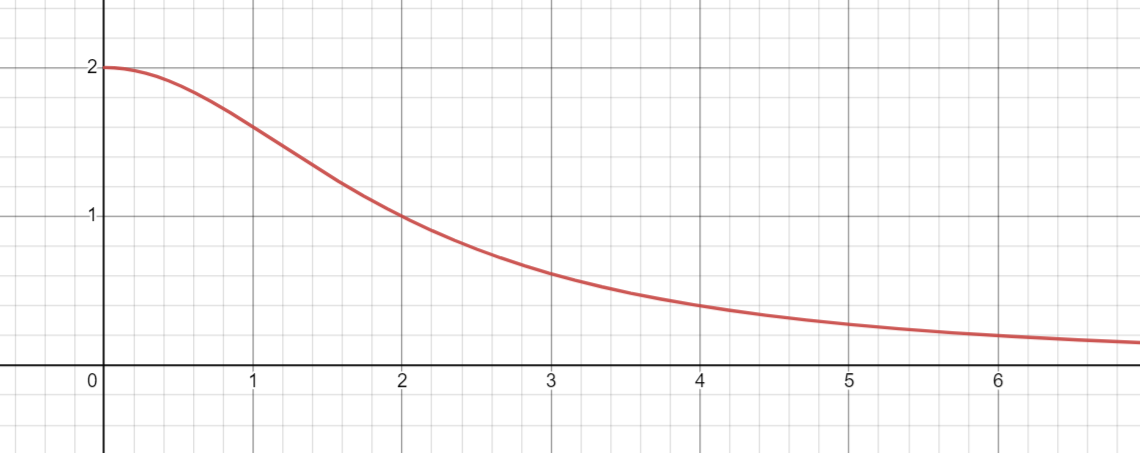
\includegraphics[scale=0.6]{NoMass.PNG}
    \centering
    \caption{An example plot of $V_\text{eff}$ with $M=0$.}
    \label{fig1}
\end{figure}

\section*{Problem 6}
Using the chain rule to turn $\dd r /\dd\tau$ into $\dd r/ \dd \phi$, along with equation (1) above, we can determine a differential equation for the shape of orbits:
\begin{alignat*}{3}
    & & \dv{r}{\tau} &= \dv{r}{\phi}\dv{\phi}{\tau} \\
    & &  &= \dv{r}{\phi}\frac{-l}{r^2 + b^2} \\
    &\implies \quad & \mathcal{E} &= \frac{1}{2}\left(\dv{r}{\phi}\frac{-l}{r^2 + b^2}\right)^2 + V_\text{eff}(r) \\
    &\implies \quad & \dv{r}{\phi} &= \pm \frac{r^2 + b^2}{l}\sqrt{2(\mathcal{E} - V_\text{eff})} \\
\end{alignat*}
See the attached python notebook for an attempted application of the Runge-Kutta method for integrating this equation.

\section*{Problem 7}
\[ V_\text{eff}(r) = \frac{-1}{\sqrt{r^2 + 1}} + \frac{25}{2(r^2 + 1)} - \frac{25}{(r^2 + 1)^\frac{3}{2}} \]
Minimum occurs ar $r \approx 21.5$ Bound orbits exist.
\begin{figure}[h]
    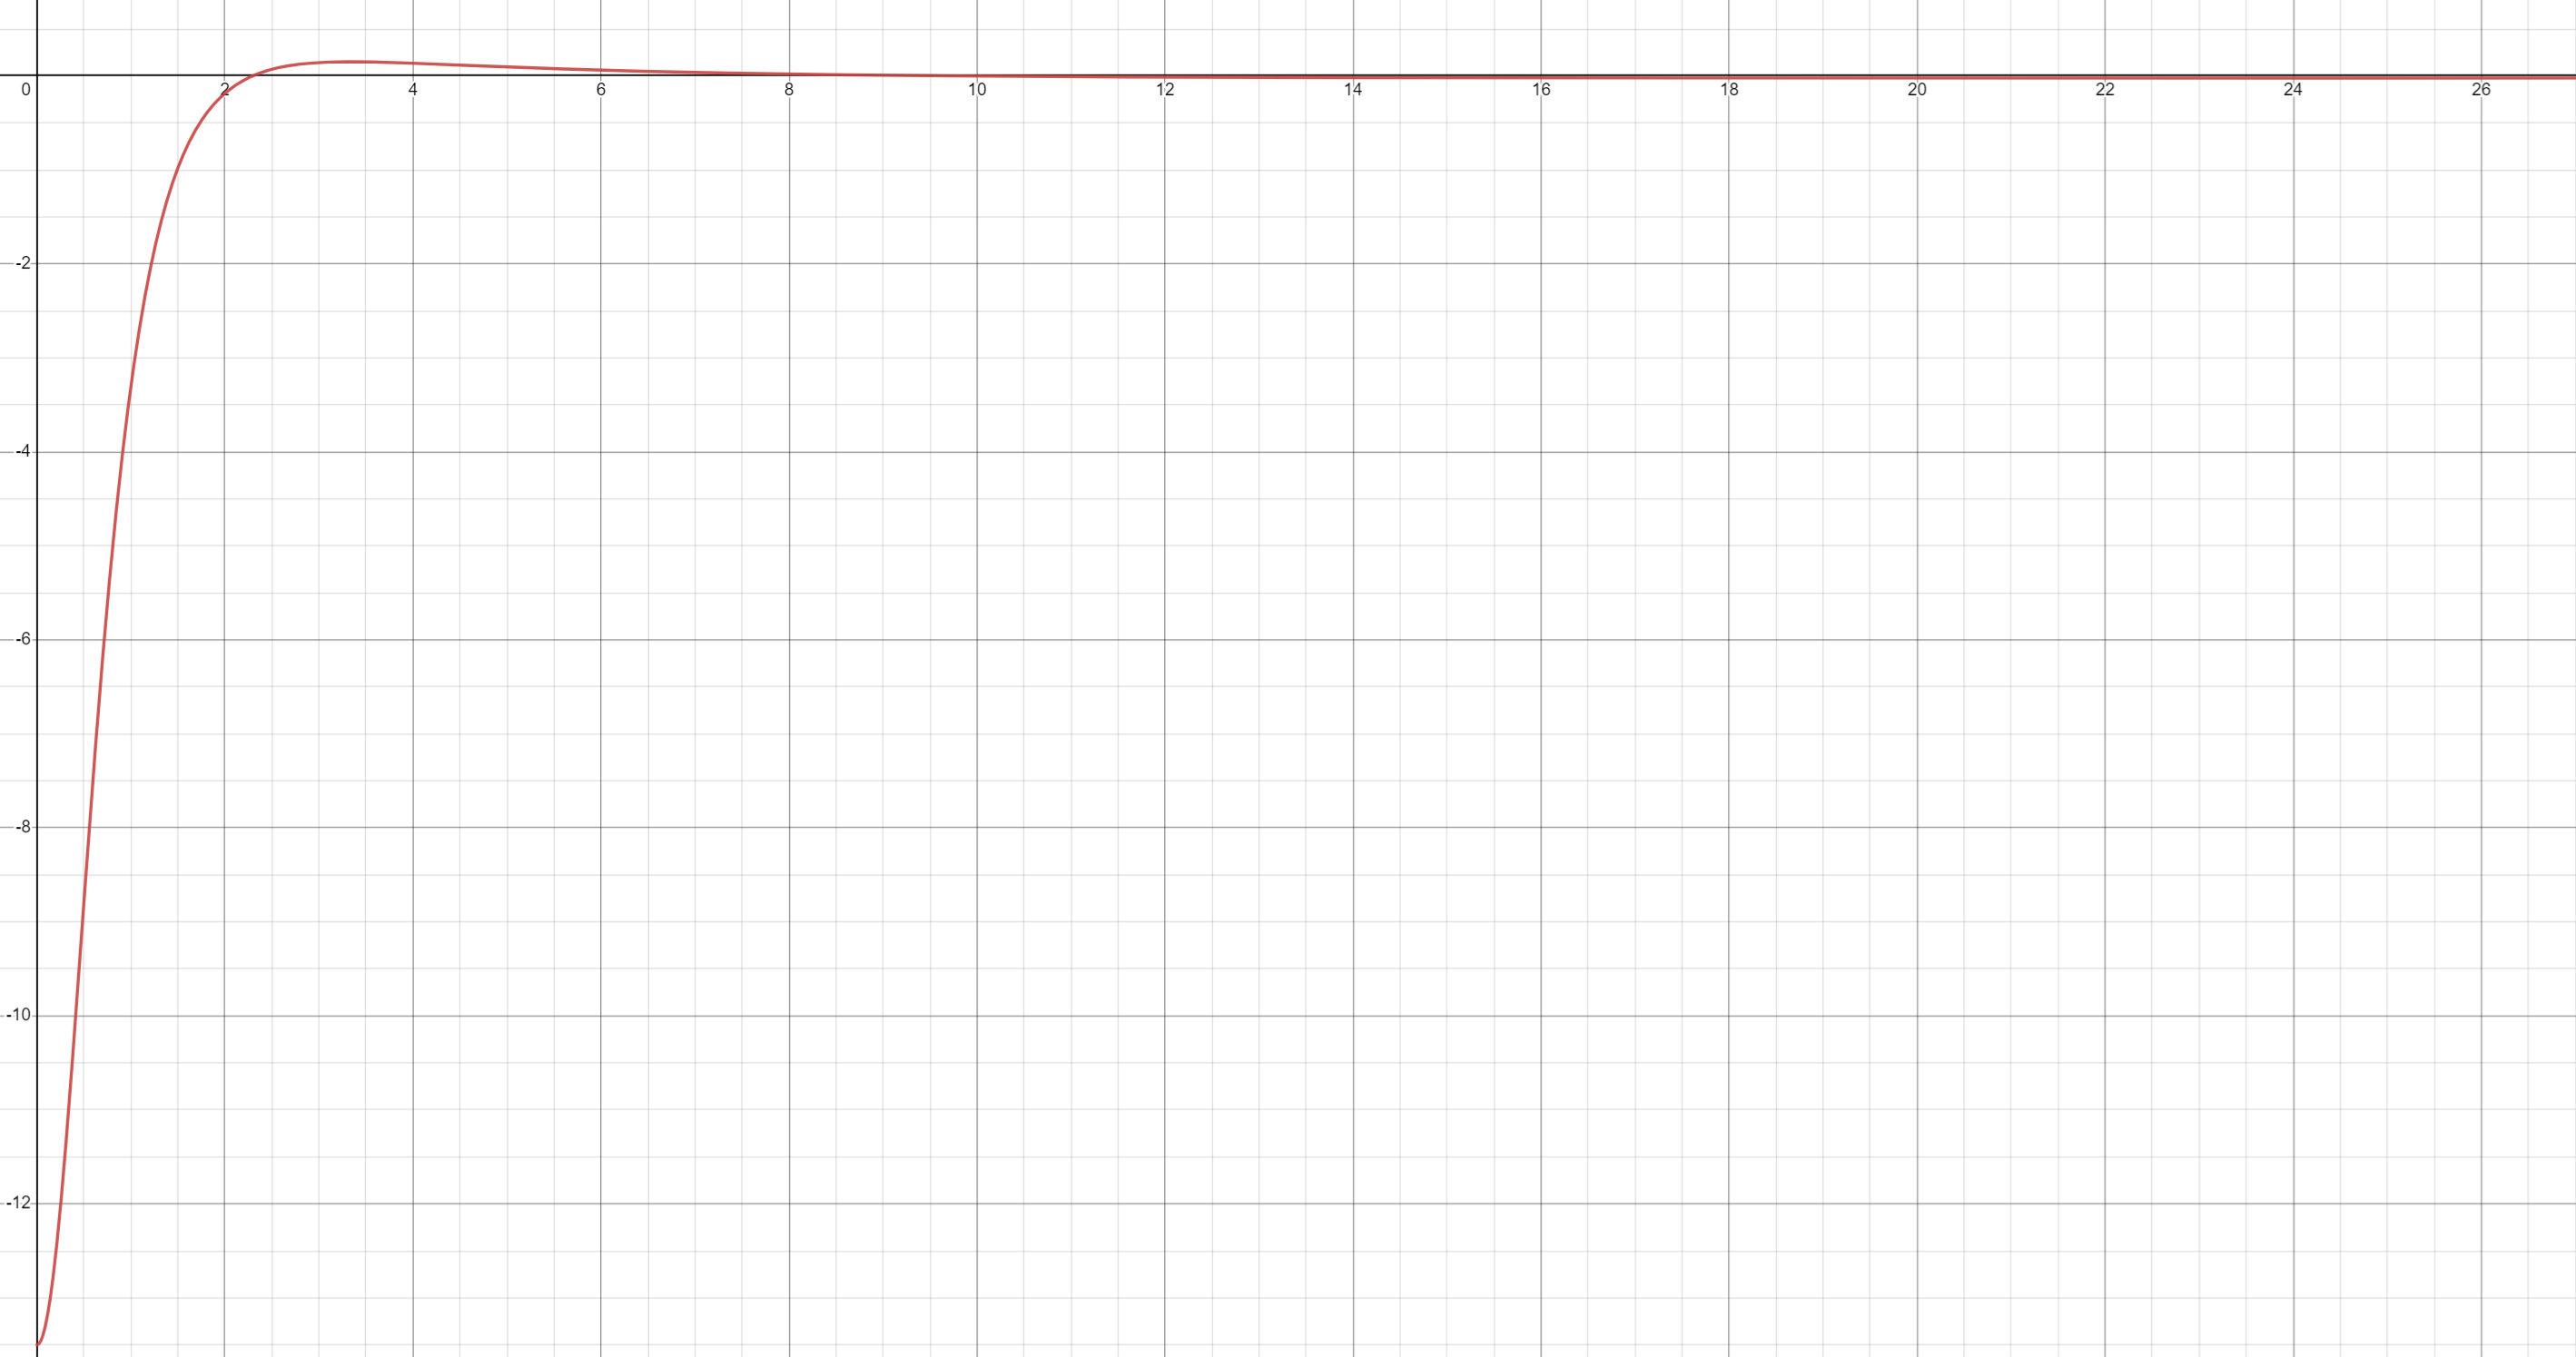
\includegraphics[scale=0.25]{prob7.PNG}
    \centering
    \caption{$V_\text{eff}(r)$ with $M=1$, $b=1$, $l=5$.}
    \label{fig2}
\end{figure}

\section*{Problem 8}
\[ V_\text{eff}(r) = \frac{-1}{\sqrt{r^2 + 9}} + \frac{4}{2(r^2 + 9)} - \frac{4}{(r^2 + 9)^\frac{3}{2}} \]
$V_\text{eff} = \mathcal{E}$ when $r \approx 17.8$. With $\mathcal{E} = -0.05$, orbits will not extend beyond this maximum radius.
\begin{figure}[h]
    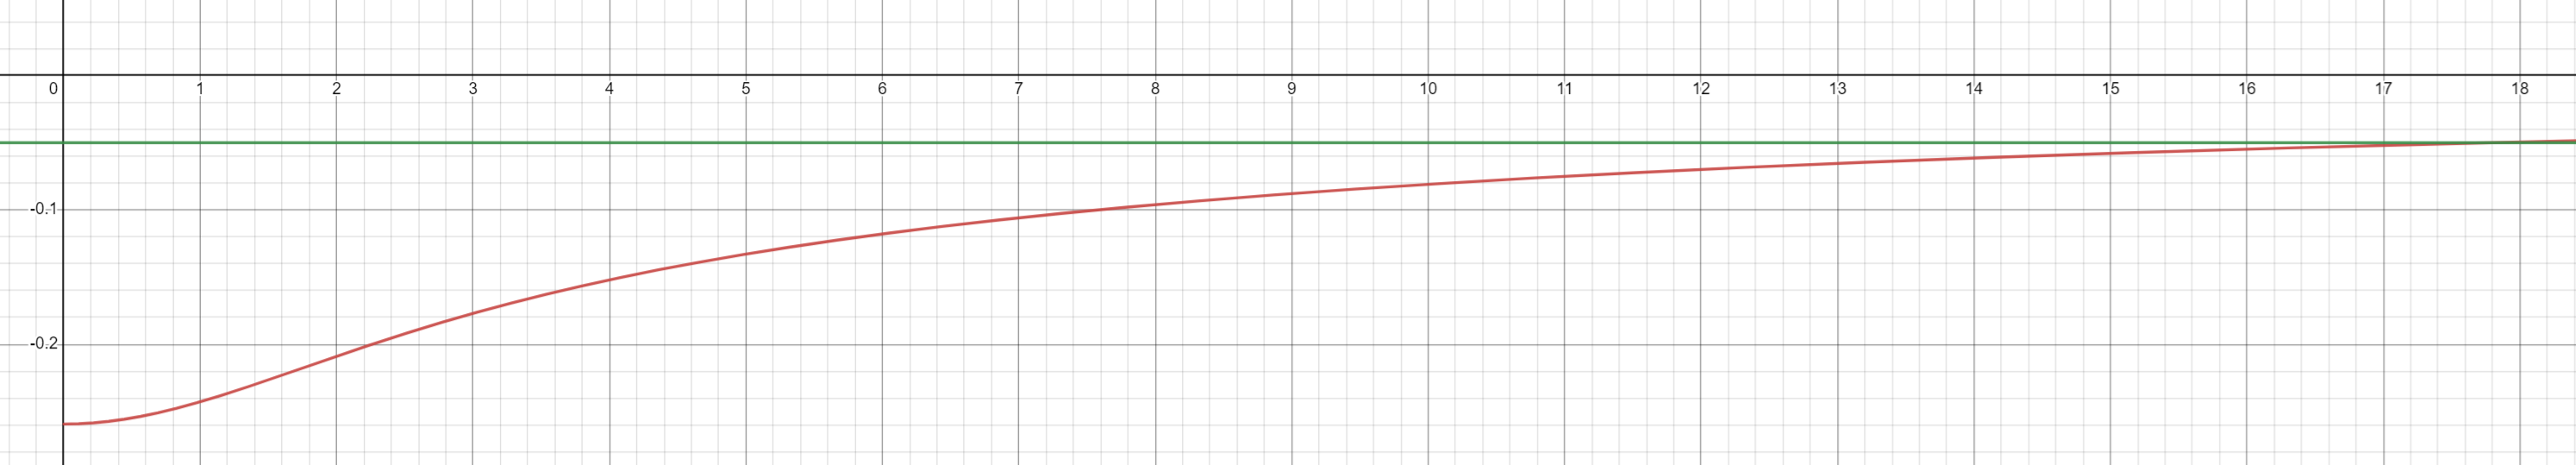
\includegraphics[scale=0.3]{prob8.PNG}
    \centering
    \caption{$V_\text{eff}(r)$ with $M=1$, $b=3$, $l=2$.}
    \label{fig3}
\end{figure}

\section*{Numeric Integration}
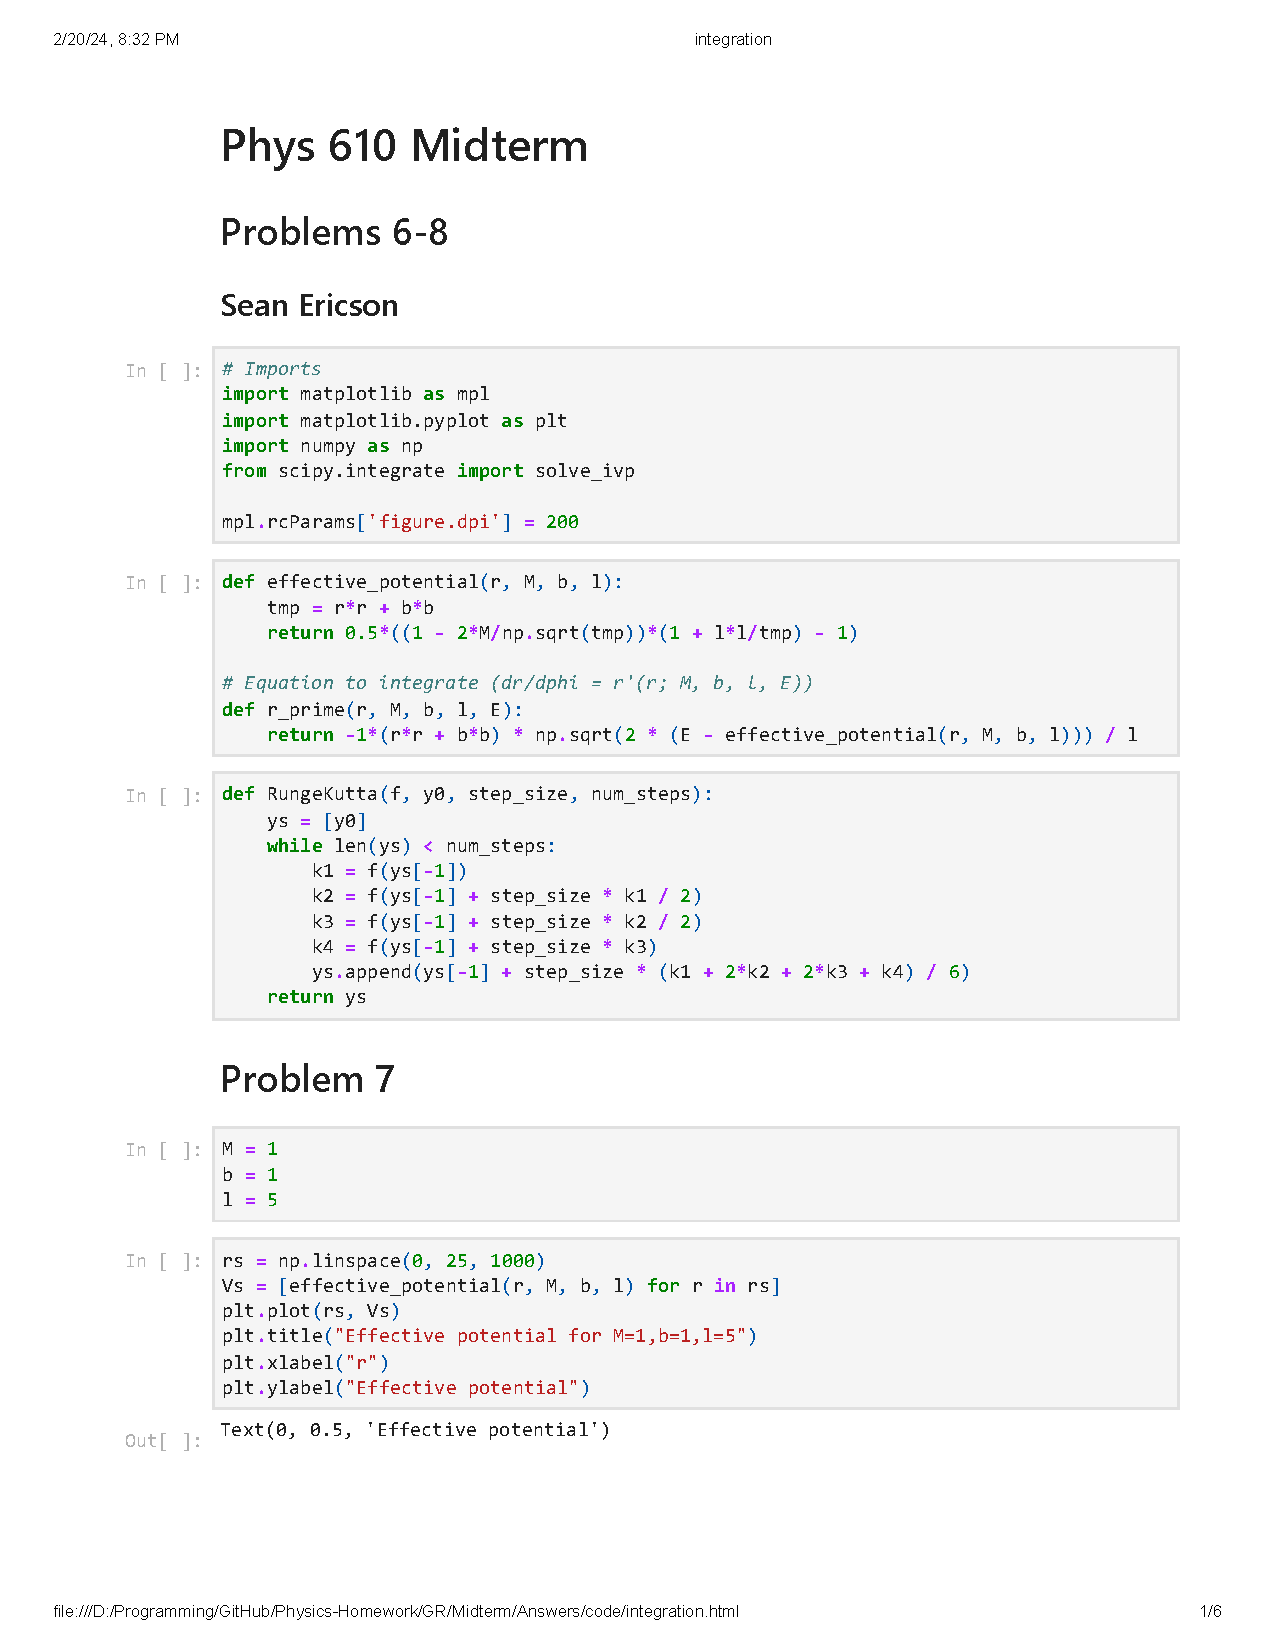
\includepdf[pages=-]{integration.pdf}

\section*{Calculations}
\includepdf[pages=-]{calcs.pdf}

\end{document}